\section{Méthodes d'impacts}
\subsection{ACV sociale}
\label{annexe_SLCA_method}
%  \colorbox{yellow}{en annexes ou traduction et commentaire !}
Insertion depuis \ref{annexe_SLCA_method_retour}.
Extrait de \citetitle{jorgensen_methodologies_2008}~\cite[Table 1: Impact categories and indicators at midpoint level]{jorgensen_methodologies_2008}.
{\scriptsize
  \begin{enumerate}
   \item Human rights
	\begin{itemize}
	\item Non-discrimination, including indicators on diversity, such as composition of employees on all levels according to gender, age group, disabled, part-time workers and other measures of diversity 
	\item Freedom of association and collective bargaining 
	\item Child labour, including hazardous child labour 
	\item Forced and compulsory labour
	\end{itemize}
  \item Labour practices and decent work conditions 
       \begin{itemize}
        \item Wages, including equal remuneration on diverse groups, regular payment, length and seasonality of work and minimum wages
        \item Benefits, including family support for basic commodities and workforce facilities 
	\item Physical working conditions, including rates of injury and fatalities, nuisances, basal facilities and distance to workplace 
	\item Psychological and organisational working conditions, such as maximum work hours, harassments, vertical, two-way communication channels, health and safety committee, job satisfaction, and worker contracts
	\item Training and education of employees
       \end{itemize}
  \item Society
      \begin{itemize}
	\item Corruption, including incidents/press reports concerning fraud, corruption and illegal price-fixing, and violation of property rights.
	\item Development support and positive actions towards society, including job creation, support of local suppliers, general support of developing countries, investments in research and development, infrastructure, and local community education programmes 
	\item Local community acceptance, such as complaints from society, and presence of communication channels 
	\item Ensuring of commitment to sustainability issues from and towards business partners 
      \end{itemize}
  \item Product responsibility 
      \begin{itemize}
      \item Integration of costumer health and safety concerns in product, such as content of contaminants/nutrients, other threats/benefits to human health (including special groups) due to product use, and complaint handling system
      \item Information about product to users, such as labelling, information about ingredients, origin, use, potential dangers, and side effects. 
      \item Marketing communications, such as ethical guidelines for advertisements 
      \end{itemize}
  \end{enumerate}
  }
\figbox{Nous retrouvons dans cet classification les thèmes de l'ACV social que nous pourrions sysnthétiser en \textbf{distribution des droits et ressources}.}

\subsection{Confrontation et sélection des méthodes d'impacts actuelles}

Certains articles font la comparaison de différentes méthodes sur un cas d'étude.
L'article de OWSIANIAK\cite{owsianiak_impact_2014} traite de modèles de fenêtres.
La conclusion est que les résultats sont globalement similaire.
Mais une attention particulière doit être portée sur les catégories~:
\begin{itemize}
\item ionizing radiation 
\item land use 
\item \emph{\textsc{et tous les impacts liés à la toxicité !}}
\end{itemize}
Cela fait tout de même une aire de protection sur trois si l'on considère la toxicité envers l'homme.
Et deux sur trois aires de protection sont sensibles en considérant l'éco-toxicité.
Ne faut-il pas jugé que les conclusions ``similaires'' des différentes méthodes sont propres à un cas d'étude.
Il n'y a comparaison que des caractérisations.

Sur quelle base les indicateurs sont-ils retenu actuellement~?
Nous cherchons évidement des éléments de réponse dans \citetitle{european_commission_characterisation_2012}~\cite{european_commission_characterisation_2012}
    
{\scriptsize
%    \begin{table}[h]
%	  \begin{center}
	     \begin{longtable}{|p{5.5cm}|p{1.2cm}|p{3cm}|p{2.8cm}|}
	      \hline
		LCIA method & Recom-mendation Level & Flow property* & Unit group data set (with reference unit)\\
	      \hline
	      ILCD2011; Climate change; midpoint; GWP100; IPPC2007&I&Mass CO2-equivalents&Units of mass (kg)\\
	      ILCD2011; Climate change; endpoint - human health; DALY; ReCiPe2008&interim&Disability Adjusted Life Years (DALY)&Units of time (a)\\
	      ILCD2011; Climate change; endpoint - ecosystems; PDF; ReCiPe2008&interim&Potentially Disappeared 5 number of species*time&Units of items*time (1*a) \\
	      ILCD2011; Ozone depletion; midpoint; ODP; WMO1999&I&Mass CFC-11-equivalents&Units of mass (kg)\\
	      ILCD2011; Ozone depletion; endpoint - human health; DALY; ReCiPe2008&interim&Disability Adjusted Life Years (DALY)&Units of time (a)\\
	      ILCD2011; Cancer human health effects; midpoint; CTUh; USEtox&II/III&Comparative Toxic Unit for human (CTUh)&Units of items (cases)\\
	      ILCD2011; Non-cancer human health effects; midpoint; CTUh; USEtox&II/III&Comparative Toxic Unit for human (CTUh)&Units of items (cases)\\
	      ILCD2011; Cancer human health effects; endpoint; DALY; USEtox&II/interi m&Disability Adjusted Life Years (DALY)&Units of time (a)\\
	      ILCD2011; Non-cancer human health effects; endpoint; DALY; USEtox&interim&Disability Adjusted Life Years (DALY)&Units of time (a)\\
	      ILCD2011; Respiratory inorganics; midpoint; PM2.5eq; Rabl and Spadaro (2004) and Greco et al (2007)&I&Mass PM2.5-equivalents&Units of mass (kg)\\
	      ILCD2011; Respiratory inorganics; endpoint; DALY; Humbert et al (2009)&I/II&Disability Adjusted Life Years (DALY)&Units of time (a)\\
	      ILCD2011; Ionizing radiation; midpoint - human health; ionising radiation potential; Frischknecht et al. (2000)&II&Mass U235-equivalents&Units of mass (kg)\\
	      ILCD2011; Ionizing radiation; midpoint - ecosystem; CTUe; Garnier-Laplace et al (2008)&interim&Comparative Toxic Unit for ecosystems (CTUe) * volume * time&Units of volume*time 3 (m *a)\\
	      ILCD2011; Ionizing radiation; endpoint- human health; DALY; Frischknecht et al (2000)&interim&Disability Adjusted Life Years (DALY)&Units of time (a)\\
	      ILCD2011; Photochemical ozone formation; midpoint - human health; POCP; Van Zelm et al. (2008)&II&Mass C2H4-equivalents&Units of mass (kg)\\
	      ILCD2011; Photochemical ozone formation; endpoint - human health; DALY; Van Zelm et al. (2008)&II&Disability Adjusted Life Years (DALY)&Units of time (a)\\
	      ILCD2011; Acidification; midpoint; Accumulated Exceedance; Seppala et al 2006, Posch et al (2008);&II&+ Mole H -equivalents&Units of mole\\
	      ILCD2011; Acidification terrestrial; endpoint; PNOF; Van Zelm et al (2007)&interim&Potentially not occurring numer of plant species in terrestrial ecosystems * time&Units of items*time (1*a)\\
	      ILCD2011; Eutrophication terrestrial; midpoint; Accumulated Exceedance; Seppala et al.2006, Posch et al 2008&II&Mole N-equivalents&Units of mole\\
	      ILCD2011; Eutrophication freshwater; midpoint;P equivalents; ReCiPe2008&II&Mass P-equivalents&Units of mass (kg)\\
	      ILCD2011; Eutrophication marine; midpoint;N equivalents; ReCiPe2008&II&Mass N-equivalents&Units of mass (kg)\\
	      ILCD2011; Eutrophication freshwater; endpoint;PDF; ReCiPe2008&interim&Potentially Disappeared number of freshwater species * time&Units of items* time (1*a)\\
	      ILCD2011; Ecotoxicity freshwater; midpoint; CTUe; USEtox&II/III&Comparative Toxic Unit for ecosystems (CTUe) * volume * time&Units of volume*time 3 (m *a)\\
	      ILCD2011; Land use; midpoint; SOM;Mila i Canals et al (2007)&III&Mass deficit of soil organic carbon&Units of mass (kg)\\
	      ILCD2011; Land use; endpoint; PDF; ReCiPe2008&interim&Potentially Disappeared Number of species in terrestrial ecosystems * time&Units of items*time (1*a)\\
	      ILCD2011; Resource depletion - water; midpoint; freshwater scarcity; Swiss Ecoscarcity2006&III&Water consumption equivalent&3 Units of volume (m )\\
	      ILCD2011; Resource depletion- mineral, fossils and renewables; midpoint;abiotic resource depletion; Van Oers et al (2002)&II&Mass Sb-equivalents&Units of mass (kg)\\
	      ILCD2011; Resource depletion- mineral, fossils and renewables; endpoint;surplus cost; ReCiPe2008&interim&Marginal increase of costs&Units of currency 2000 (\$) \\
	      \hline
	      \caption{Recommandations ilcd. Base de la méthode d'impacts consécutive. Table extraite de \citetitle{european_commission_characterisation_2012} \cite{european_commission_characterisation_2012}.}
    	  \label{tab:methode_ilcd2011_recommendation}
	      \end{longtable}
%	  \end{center}
%  \end{table}
}
%  \figbox{
  Le recommandation table~\ref{tab:methode_ilcd2011_recommendation} est une sélection parmi les diverses méthodes pour chaque indicateur sur la base de plusieurs critères.
  Il me semble essentiel de \emph{souligner} l'imbrication du jugement en soulignant la `construction' de cette recommandation.
  \cite{jrc_ilcd_2011}
  
  \blockcquote[traduction, section 2.1.1 p23/159 du pdf (pagination p.7-8)]{jrc_ilcd_2011}{
  Les critères généraux portent séparément sur les qualités scientifiques et sur l'\emph{acceptation} par les parties prenantes et l'\emph{applicabilité} aux ensembles de données LCI.
  
  \textbf{Les critères scientifiques}
  \begin{enumerate}
    \item Exhaustivité du périmètre
    \item \emph{Pertinence} environnementale
    \item Robustesse et certitude scientifique
    \item Documentation, transparence et reproductibilité
    \item \emph{Applicabilité}
  \end{enumerate}
  
  \textbf{Critère d'acceptation des parties prenantes}
  
  Degré d'acceptation des parties prenantes et l'\emph{aptitude à la communication dans une \textbf{entreprise} et des contextes politiques}.
  
  Chaque critère est défini par un certain nombre de sous-critères.
  \ldots
  Des critères spécifiques
  Avant d'élaborer les critères spécifiques, le mécanisme environnemental de la catégorie d'impact en question a été décrite avec un diagramme comportant toutes les voies et les flux \emph{pertinents} qui pourraient être inclus dans un modèle de caractérisation.
  Sur la base de l'analyse des méthodes et soutenu par le diagramme, \emph{un nombre limité de critères supplémentaires de sous-catégories spécifiques ont été développées dans les deux critères}:
  «\emph{Pertinence} environnementale» et «robustesse scientifique et certitude» pour compléter les critères généraux et de les adapter aux spécificités de la catégorie d'impact, la capture des caractéristiques centrales de cette catégorie et les points décisifs sur lesquels les méthodes de caractérisation analysées diffèrent, soutenant ainsi la discrimination entre les différentes méthodes.
  
  Une description détaillée des critères et sous-critères est donnée dans le document sur le cadre et les exigences de l'évaluation d'impact en cycle de vie (LCIA, Life cycle impact assessment).
  [\ldots]
  Afin de soutenir une évaluation globale, un score pour chaque critère est développé sur la base d'une évaluation de la notation des sous-critères.
  Pour les critères scientifiques, un score global est ensuite développé sur la base de la notation de chaque critère de la science sur la base.
  \emph{La compilation des résultats est basée sur ``un jugement d'expert''}, y compris l'examen de l'\textbf{importance} \textbf{des} \textbf{différents} \textbf{critères} \textbf{et} \textbf{sous-critères}.
  Les états résultant sur les critères scientifiques sur la base et sur le critère d'acceptation des parties prenantes sont les bases des recommandations finales de la méthode.
  Les résultats de l'évaluation sont résumés dans les recommandations sur la méthode de caractérisation pour chaque catégorie d'impact.
%  General criteria
%  The general criteria focus separately on scientific qualities and on stakeholder acceptance and applicability to LCI data sets.
%  
%  Scientific criteria
%  1. Completeness of scope
%  2. Environmental relevance
%  3. Scientific robustness and certainty
%  4. Documentation, transparency and reproducibility
%  5. Applicability
%  
%  Stakeholder acceptance criterion
%  6. Degree of stakeholder acceptance and suitability for communication in a business
%  and policy contexts
%  
%  Each criterion is specified through a number of sub criteria.
%  
%  Specific criteria
%  Prior to developing the specific criteria, the environmental mechanism of the impact category in question was described with a flow diagram with all relevant pathways and flows which might be included in a characterisation model.
%  Based on the methods analysis and supported by the diagram, a limited number of additional category-specific sub criteria were developed under the two criteria:
%  ‘Environmental relevance’ and ‘Scientific robustness and certainty’ to complement the general criteria and adapt them to the specificities of the impact category, capturing the central characteristics of that category and the decisive points at which the analysed characterisation methods differ and thus supporting discrimination between the different methods.
%  
%  A detailed description of criteria and sub criteria is given in the LCIA- Framework and requirements document.
%  The detailed assessment of the characterisation methods for each impact category is provided in separate spreadsheets 8 .
%  The spreadsheets were used as supporting working documents during the expert judgement processes.
%  For each criterion and sub criterion a score was assigned to the characterisation models reflecting the compliance of the model with the criterion or sub criterion requirements.
%  
%  The used score are provided below:
%  A: Full compliance
%  B: Compliance in all essential aspects
%  C: Compliance in some aspects
%  D: Little compliance
%  E: No compliance
%  
%  For the overall evaluation of the characterisation model, the importance of each criterion and sub criterion needs to be assessed for the impact category in question.
%  A differentiation between normal (N) and high (H) importance is applied.
%  Criteria of high importance are criteria which address fundamental aspects of significance for the resulting characterisation factors.
%  Some of the sub criteria are so important that an exclusion threshold is defined as a required minimum performance below which the characterisation model will not be considered any further in the analysis.
%  Whenever a characterisation model fails to pass such an exclusion threshold, the analysis of that characterisation model stops.
%  In order to support an overall evaluation, a score for each criterion is developed based on an evaluation of the scoring of the sub-criteria.
%  For the science based criteria, an overall score is then developed based on the scoring of each science based criterion.
%  The compilation of the scores is based on “expert judgement” including consideration of the importance of different criteria and sub criteria.
%  The resulting statements on the science based criteria and on the stakeholder acceptance criterion are the bases of the final method recommendations.
%  The findings from the evaluation are summarized in recommendations on the characterisation method for each impact category.
  }
  
  En sommes des jugements de \emph{pertinence}, d'\emph{acceptabilité} et d'\emph{importance} à de nombreux étages, font obstacle à une réelle appropriation par chaque décideur.
  
  
%  xxxxxxxxxxxxxxxxxxxxxxxxxxxxxxxxxxxxxxxxxxxxxxxxx
%   
%  
%  \colorbox{yellow}{à relocaliser ! pas que de la biblio}
  
    
%    La sélection de la méthode d'évaluation des impacts doit prendre en compte les spécificités propres à l'étude et les valeurs ou intention d'évaluation du décisionnaires.
%    Des descriptifs des méthodes ainsi que les recommandations européennes sont disponibles dans les publications du JRC\cite{jrc_ilcd_2011}.
%    Il a été rappelé à Lille lors du Congrès ACV 2013 que le traitement des ressources diffère suivant les méthodes d'impact\cite{sonnemann_criticality_2013, adibi_introducing_2013}.

La comparaison de méthodes entres-elles fait apparaître des nuances en nombres de substances suivies et en compartiment observés.

Qu'en est-il de l'influence du nombre d'indicateurs par thème.
IMPACT 2002+, ReCiPe 2008 and l'ILCD 2011~?~\cite{jolliet_impact_2003, goedkoop_recipe_2009}
    {\scriptsize
%    \begin{table}[h]
%    \begin{center}
%    \caption{Comparatif des méthodes IMPACT 2002+ et ReCiPe 2008.}
    \begin{longtable}{ l p{3cm} l l p{3cm} l}
    \hline
    18 & ReCiPe2008 & Unité & 15 & IMPACT2002+ & Unité  \\
    \hline
    1&Climate change&kg CO2 eq&13&Global warming&kg CO2 eq\\
    2&Ozone depletion&kg CFC-11 eq&5&Ozone layer depletion&kg CFC-11 eq\\
    3&Terrestrial acidification&kg SO2 eq&9&Terrestrial&kg SO2 eq\\
    &&&&acidification/nutrification\\
    &ABS -> &&11&Aquatic acidification&kg SO2 eq\\
    4&Freshwater eutrophication&kg P eq&12&Aquatic eutrophication&kg PO4 P-lim\\
    5&Marine eutrophication&kg N eq&&<- Sous-compartimenté&\\
    6&Human toxicity&kg 1,4-DB eq&1&Carcinogens&kg C2H3Cl eq\\
    &Sous-compartimenté -> &&2&Non-carcinogens&kg C2H3Cl eq\\
    7&Photochemical oxidant&kg NMVOC&6&Respiratory organics&kg C2H4 eq \\
    &formation\\
    8&Particulate matter formation&kg PM10 eq&3&Respiratory inorganics&kg PM2.5 eq\\
    9&Terrestrial ecotoxicity&kg 1,4-DB eq&8&Terrestrial ecotoxicity&kg TEG soil\\
    10&Freshwater ecotoxicity&kg 1,4-DB eq&7&Aquatic ecotoxicity&kg TEG water\\
    11&Marine ecotoxicity&kg 1,4-DB eq&&<- Sous-compartimenté&\\
    12&Ionising radiation&kBq U235 eq&4&Ionizing radiation&Bq C-14 eq\\
    13&Agricultural land occupation&m2a&10&Land occupation&m2org.arable\\
    14&Urban land occupation&m2a&&<- Sous-compartimenté&\\
    15&Natural land transformation&m2&&<- ABS&\\
    16&Water depletion&m3&&<- ABS&\\
    17&Metal depletion&kg Fe eq&15&Mineral extraction&MJ surplus\\
    18&Fossil depletion&kg oil eq&14&Non-renewable energy&MJ primary\\
    \hline
    \caption{Comparatif des méthodes IMPACT 2002+ et ReCiPe 2008.}
        \label{tab:ReCiPe2008 - IMAPCT2002+}
    \end{longtable}
%    \end{center}
%    \end{table}
    }
    \figbox{
    Dans la table~\ref{tab:ReCiPe2008 - IMAPCT2002+}, deux méthodes sont confrontée.
    Le nombre d'impacts est comptabilisé et les indicateurs de IMPACT2002+\footnote{
    Les 15 indicateurs de \textsc{Impact}2002+ sont tirés de la table 1 de la publication.
    On y distingue, bien que sur la même ligne, la toxicologie cancérigène et non-cancérigène.
    La figure de la publication ne comporte que 14 indicateurs~\cite{jolliet_impact_2003}.}
    sont positionnés en face de leurs homologues de ReCiPe2008~\cite{goedkoop_recipe_2013} mais conservent leur numéro d'ordre dans la présentation initiale~\cite{jolliet_impact_2003}.
    }
%    xxxxxxxxxxxxxxxxxxxxxxxxxxxxxxxxxxxxxxxxxxxxxxxxx
  %   owsianiak_impact_2014,
%  	À COMPLÉTER
% total impact scores aller cherche le support électronique complémentaire !
%    
%    xxxxxxxxxxxxxxxxxxxxxxxxxxxxxxxxxxxxxxxxxxxxxxxxx
    Sur une comparaison plus étendue il est également intéressant d'observer la cible des indicateurs.
    La sélection des méthodes indicateurs a un rôle important dans l'interprétation consécutive.
    Je relève un caractère très anthropocentrique de l’ACV.
    
    \begin{wrapfigure}{i}{0.4\textwidth}
      	\centering
      	\caption{Trichotomie des aires de protection sur les indicateurs midpoint.}
      	\vspace{-12pt}
      	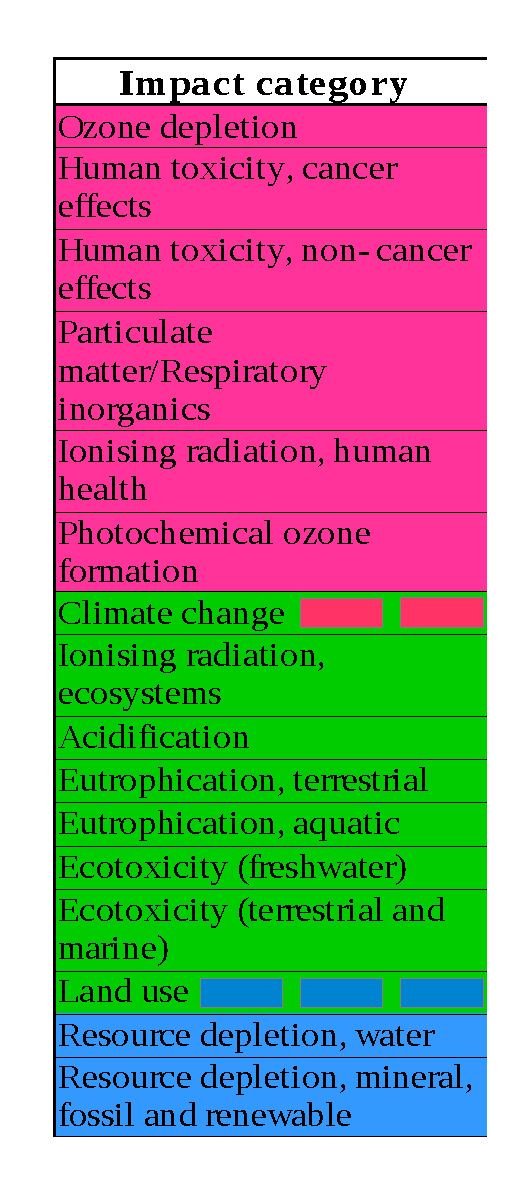
\includegraphics[width=0.37\textwidth]{/home/rudy/Documents/rudy/01_These/11_production/01_COMMUNICATION/figures/trichotomie_midpoint.pdf}
      	\label{fig:Trichotomie_mipoint}   
      \end{wrapfigure}
      
    La méthode \textsc{impact}2002+ par exemple, dans la 
    \blockcquote{jolliet_impact_2003}{
    Fig. 1: Overall scheme of the IMPACT 2002+ framework, linking LCI re-
    sults via the midpoint categories to damage categories, based on Jolliet et
    al. (2003a)
    }
    comporte 14 indicateurs midpoint.
    Elle les répartie sur 4 aires de protection, Santé Humaine, Qualité des Ecosystème, Changement Climatique et Ressources.
    Au total 7 indicateurs midpoint alimentent les aires Santé Humaine (5) et Ressources (2).
    Cette lecture indique que pour moitié, les indicateurs de ce type d’analyse vise à garantir la santé et la richesse de l’Homme.
    L’autre moitié de l’analyse vise à garantir la viabilité de l’écosystème (sa stabilité)
    \footnote{Étonnamment selon cette représentation l’écosystème ne comporte pas d’autre fraction d’espèce, mammifère par exemple, ou encore les espèces utilisées dans les protocoles toxicologiques, concernés par les problématiques respiratoires des particules ou les dommages des radiations ionisantes.}.
  %  \colorbox{red}{! pb de copyright à vérifier}
%  
  % \begin{figure}[h]
  % \begin{center}
  %  \includegraphics[width=10cm]{/home/rudy/Documents/rudy/01_These/11_production/01_COMMUNICATION/figures_extraites/schema_impact_2002.pdf}
  % \end{center}
  % \caption{Schéma global du modèle, depuis l'inventaire aux aires de protection de la méthode IMPACT2002+.
  % Des mécanismes environnementaux plus incertains ou évalués qualitativement (flèches en pointillés) indiquent que des indicateurs visant l’aire de la santé humaine visent « potentiellement » la qualité de l’écosystème.}
  % \label{fig:impact2002_method_schema}
  %  \end{figure}
    Une construction similaire se trouve dans la méthode ReCiPe.
  % \begin{figure}[ht]
  % \begin{center}
  %  \includegraphics[width=10cm]{/home/rudy/Documents/rudy/01_These/11_production/01_COMMUNICATION/figures_extraites/schema_impact_recipe.pdf}
  % \end{center}
  % \caption{Schéma global du modèle, depuis l'inventaire aux aires de protection de la méthode ReCiPe.}
  % \label{fig:RECIPE_method_schema}
  %  \end{figure}
  
On distinguera entre \textsc{Impact}2002+ et ReCiPe2008 que le changement climatique contribue à la dégradation de l'écosystème et de la santé humaine.
Plus spécifiquement la méthode ReCiPe propose l'agrégation complète en un score unique.
Cela, comme décrit dans la section multi-dimensionnalité, et au premier chapitre, n'est pas compatible avec une conception forte de la soutenabilité rejetant la compensation - substitution.
   
%    Les impacts non attribués sont restés blanc.
 

\figbox{
Ce profil de répartition entre aire de protection peut être reproduit de façon récurrente au sein des méthodes d’ACV au niveau midpoint.
C'est ce que nous représentons figure~\ref{fig:Trichotomie_mipoint}.
Nous pouvons l’illustrer en soulignant par un code de couleurs les aires de protection concernées par les impacts au sein des méthodes.
Nous avons attribué sur la base du lien midpoint – endpoint des méthodes mixtes précédemment exposées les couleurs suivantes~: Rose pour la santé humaine, bleu pour l’épuisement des ressources, vert pour l’écosystème.
Pour simplifier la lecture nous n’avons que de façon limitée représenté plusieurs couleurs pour un même impact malgré des modèles existant. Par exemple, sous ReCiPe, le changement climatique génère un dommage à la fois sur la santé humaine et sur l’écosystème. La même remarque peut être faite sur l’utilisation des sols, entre écosystème et ressource.}